\documentclass[preview]{standalone}
\usepackage{varwidth}
\usepackage[utf8x]{inputenc}
\usepackage{amsmath,amssymb,amsthm,bm,tikz}
\usetikzlibrary{automata,arrows,shapes,snakes}
\begin{document}
\begin{varwidth}{50in}
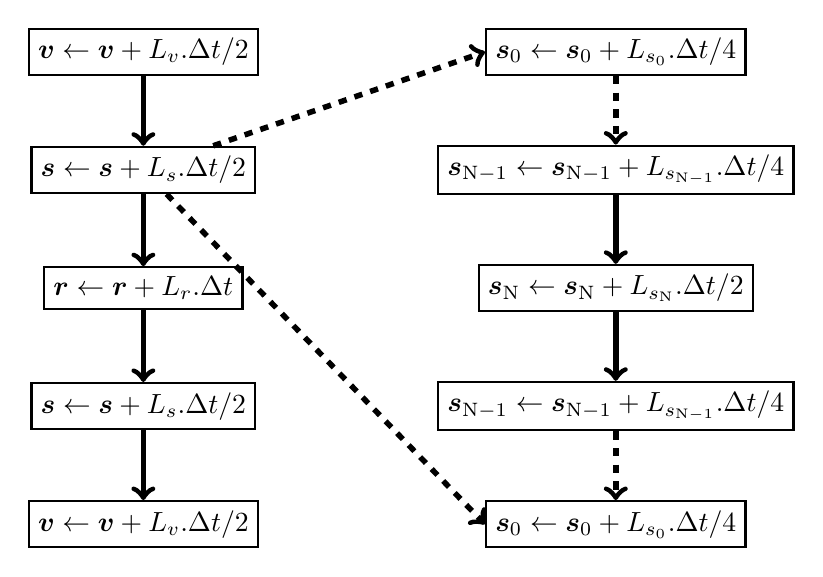
\begin{tikzpicture}

%Global
\node (v1) at (0,6.0) [draw,thick,minimum width=0.2cm,minimum height=0.2cm] { $\bm{v} \leftarrow \bm{v}+L_v.\Delta t/2$ };
\node (s1) at (0,4.5) [draw,thick,minimum width=0.2cm,minimum height=0.2cm] { $\bm{s} \leftarrow \bm{s}+L_s.\Delta t/2$ };
\node (r)  at (0,3.0) [draw,thick,minimum width=0.2cm,minimum height=0.2cm] { $\bm{r} \leftarrow \bm{r}+L_r.\Delta t$ };
\node (s2) at (0,1.5) [draw,thick,minimum width=0.2cm,minimum height=0.2cm] { $\bm{s} \leftarrow \bm{s}+L_s.\Delta t/2$ };
\node (v2) at (0,0.0) [draw,thick,minimum width=0.2cm,minimum height=0.2cm] { $\bm{v} \leftarrow \bm{v}+L_v.\Delta t/2$ };

\draw[line width=2pt, ->] (v1) -- (s1);
\draw[line width=2pt, ->] (s1) -- (r);
\draw[line width=2pt, ->] (r) -- (s2);
\draw[line width=2pt, ->] (s2) -- (v2);

%Spin
\node (s01) at (6,6.0) [draw,thick,minimum width=0.2cm,minimum height=0.2cm] {$\bm{s}_0 \leftarrow \bm{s}_0+L_{s_0}.\Delta t/4$ };
\node (sN1) at (6,4.5) [draw,thick,minimum width=0.2cm,minimum height=0.2cm] {$\bm{s}_{\rm N-1}\leftarrow\bm{s}_{\rm N-1}+L_{s_{\rm N-1}}.\Delta t/4$};
\node (sN)  at (6,3.0) [draw,thick,minimum width=0.2cm,minimum height=0.2cm] {$\bm{s}_{\rm N} \leftarrow \bm{s}_{\rm N}+L_{s_{\rm N}}.\Delta t/2$ };
\node (sN2) at (6,1.5) [draw,thick,minimum width=0.2cm,minimum height=0.2cm] {$\bm{s}_{\rm N-1}\leftarrow\bm{s}_{\rm N-1}+L_{s_{\rm N-1}}.\Delta t/4$};
\node (s02) at (6,0.0) [draw,thick,minimum width=0.2cm,minimum height=0.2cm] {$\bm{s}_0 \leftarrow \bm{s}_0+L_{s_0}.\Delta t/4$ };

\draw[line width=2pt,dashed, ->] (s01) -- (sN1);
\draw[line width=2pt, ->] (sN1) -- (sN);
\draw[line width=2pt, ->] (sN) -- (sN2);
\draw[line width=2pt,dashed, ->] (sN2) -- (s02);

%from Global to Spin
\draw[line width=2pt, dashed, ->] (s1) -- (s01.west);
\draw[line width=2pt, dashed, ->] (s1) -- (s02.west);

\end{tikzpicture}
\end{varwidth}
\end{document}
